\documentclass[a4j,12pt,dvipdfmx]{jreport}
\usepackage[top=35mm, bottom=30mm, left=30mm, right=30mm]{geometry}

% \oddsidemargin= 5mm   
% \textwidth = 160mm
% \textheight = 205mm
% \addtolength{\textheight}{3cm}
% %\addtolength{\textwidth}{1.5cm}
% \topmargin = -5mm
% \headheight = 0mm
% \footskip = 10mm

% % 図形に関する処理
\renewcommand{\topfraction}{1.0}
\renewcommand{\bottomfraction}{1.0}
\renewcommand{\dbltopfraction}{1.0}
\renewcommand{\textfraction}{0.01}
\renewcommand{\floatpagefraction}{1.0}
\renewcommand{\dblfloatpagefraction}{1.0}
\setcounter{topnumber}{5}
\setcounter{bottomnumber}{5}
\setcounter{totalnumber}{10}

\usepackage{url}
\usepackage[dvipdfmx]{graphicx}
\usepackage{amsmath,amsthm,amssymb,ascmac}
\usepackage{fancyhdr}
\usepackage{fancybox}
\usepackage{fancyvrb}
\usepackage[T1]{fontenc}
\usepackage{subcaption}
\usepackage{comment}
\usepackage{here}
\usepackage{float}
\usepackage{booktabs}
\usepackage{makecell}

\usepackage{listings,jvlisting} %日本語のコメントアウトをする場合jvlisting(もしくはjlisting)が必要
%ここからソースコードの表示に関する設定
\lstset{
    language=bash,
    basicstyle=\ttfamily\small,
    numbers=left,
    numberstyle=\tiny,
    numbersep=5pt,
    breaklines=true,
    frame=tb,
    captionpos=b
}

\begin{document}
\pagenumbering{roman}
%表紙
\begin{titlepage} \centering
  %\LARGE
  \null \null
  \vspace{10mm}
  令和04年度 卒業研究論文 付録\\
  %\vfill
  \vspace{55.15mm}
  \null
  % 研究題目\\
  {\Large CNNを用いた動画検索用インデックス作成に関する研究 マニュアル}\\
  %\vfill \vfill
  %\vfill
  
  \vspace{82.5mm}
  %{\Large 平成24年2月23日}
  %\vspace{15mm}
  
  \large
  総合工学科 情報システムコース 5年\\[1mm]
  1801113 藤田 晴斗\\[1mm]
  指導教員 総合工学科 藤原 和彦\\
  
  \vspace{16mm}
  {仙台高等専門学校}
  \null

\end{titlepage}

%目次
\tableofcontents
% \clearpage
% \clearpage \tableofcontents
\listoftables
\listoffigures
% \thispagestyle{empty}
% \pagestyle{plain}
% \setcounter{page}{0}


%\setcounter{page}{0}
%\pagenumbering{roman}
%\tableofcontents
%\thispagestyle{empty}
{\clearpage}
\large
\renewcommand{\baselinestretch}{1.1}
\appendix
\chapter{機動するまでの手順}
GitHubからソースコードをダウンロードし,Linux環境で動作させる手順を説明する.

\section{GitHubからソースコードをダウンロード}
GitHubからダウンロードする.
\begin{lstlisting}[caption=Example,escapechar=|]
  cd ~   # ホームディレクトリに移動
  git clone https://github.com/[username]/[ripository_name].git
\end{lstlisting}

\section{Python環境を構築}
仮想環境での実行を推奨する.
Anacondaを用いた.

Anacondaの仮想環境をアクティブにした状態で,必要なパッケージをインストールする.
\begin{lstlisting}[caption=hoge,label=fuga]

\end{lstlisting}

\section{動作確認}
\begin{lstlisting}[caption=hoge,label=fuga]
  cd ~/[リポジトリ名]
  conda activate [仮想環境名]
  flask run
  #ポート番号を指定する場合
  flask run --port [ポート番号]
  #ホスト名を指定する場合
  flask run --host [ホスト名]
\end{lstlisting}

\chapter{使用方法}
\label{sec:usage}
本システムの使用方法について説明する.
手順は大きく2つに分かれており,動画を解析するために事前に動画をアップロードすること,そして画像を用いた検索を行うことがそれぞれ必要となる.

本研究用のアカウントとして次を用意してある.
> ユーザー名:kaz-lab
> メールアドレス:kaz-lab@example.com
> パスワード:kaz-lab

\section{ユーザ登録}
本システムでは不特定多数のユーザができるようにするため,ユーザ情報が必要となっている.

ユーザ登録画面を図\ref{fig:user_register}に示す.

\begin{figure}[H]
  \centering
  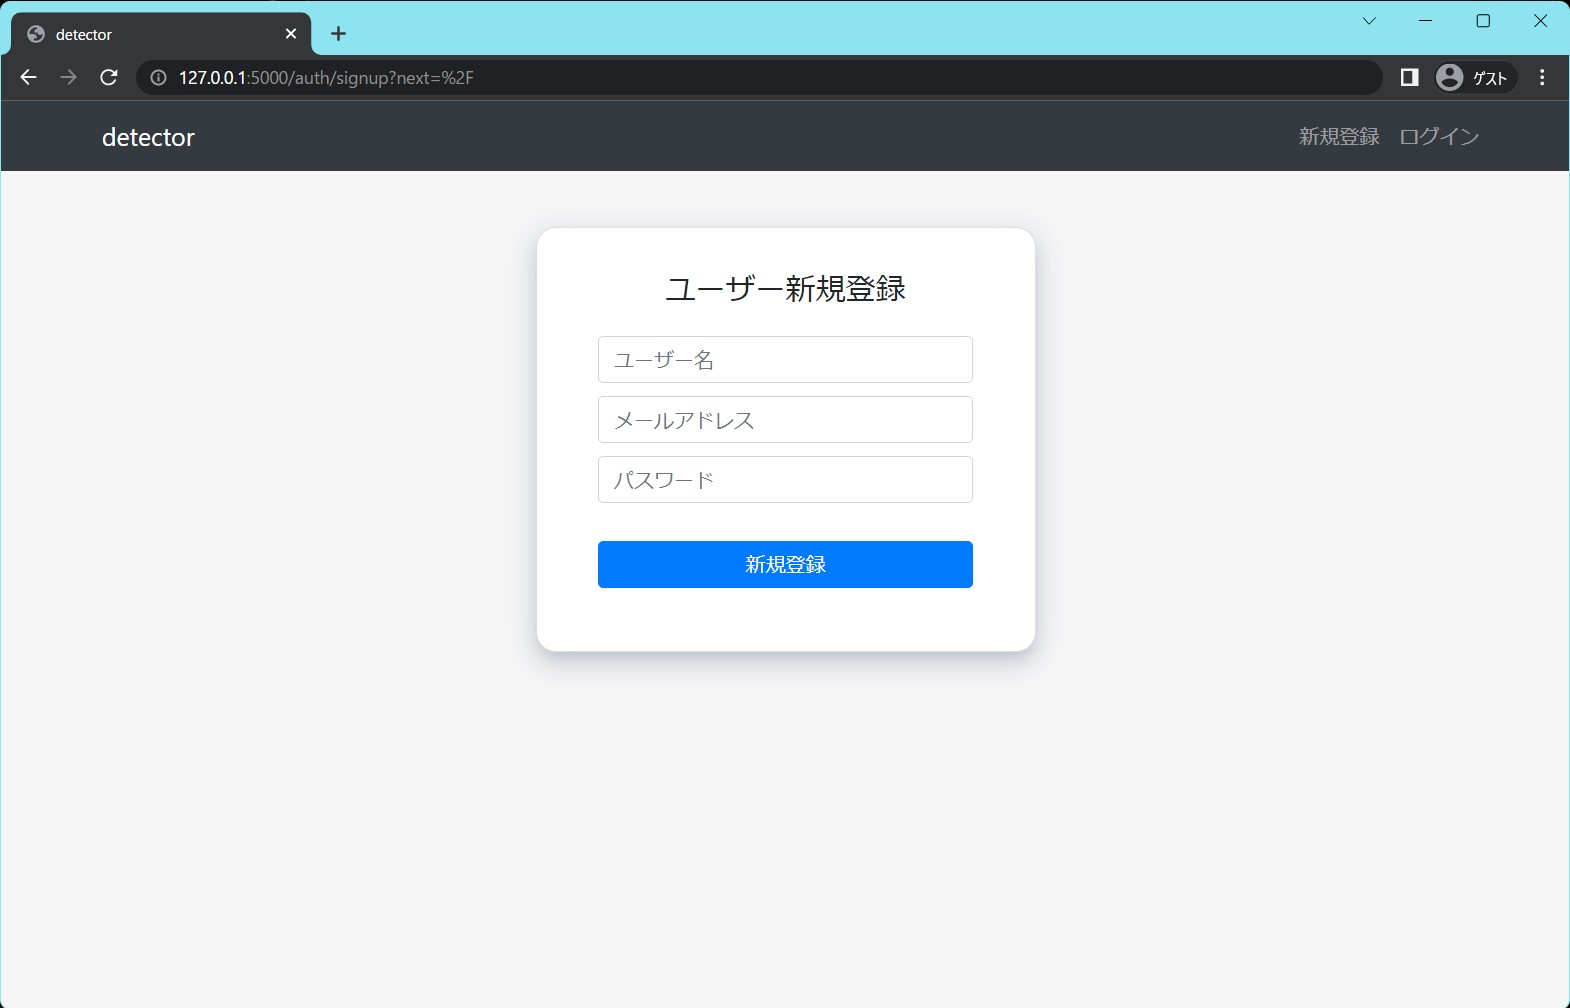
\includegraphics[width=13cm]{image/user_register.jpg}
  \caption{ユーザ登録}
  \label{fig:user_register}
\end{figure}

登録にはユーザ名,メールアドレス,パスワードを入力する.

\section{ログイン}
ログイン画面を図\ref{fig:user_login}に示す.

\begin{figure}[H]
  \centering
  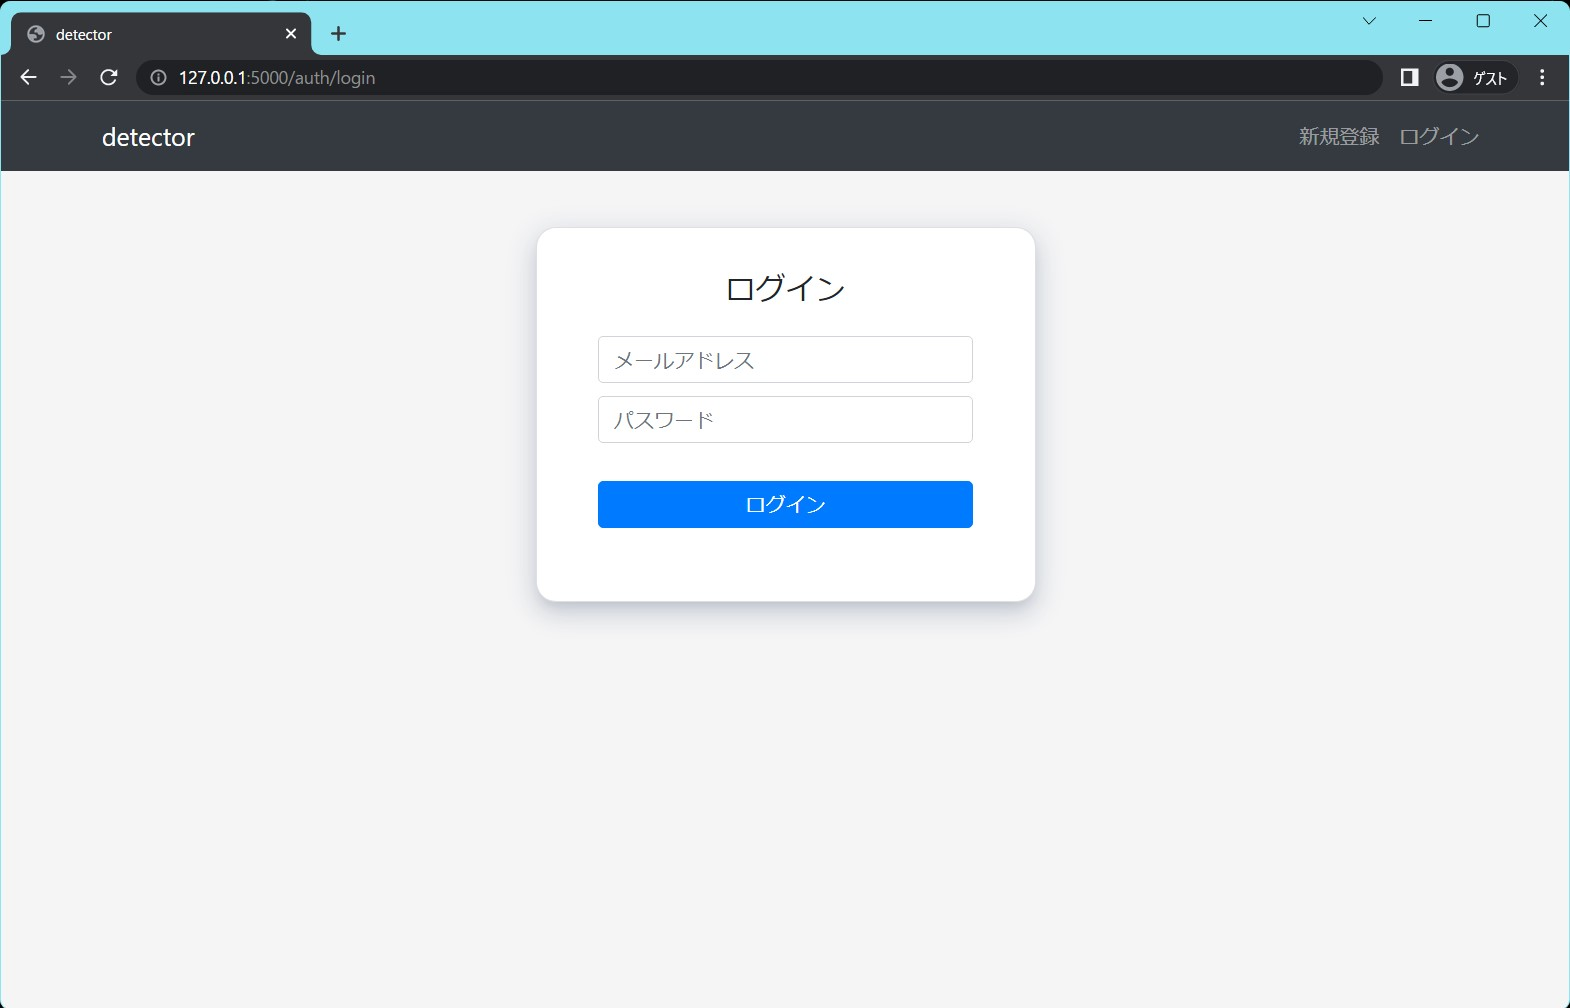
\includegraphics[width=13cm]{image/user_login.jpg}
  \caption{ログイン画面}
  \label{fig:user_login}
\end{figure}

ログインには,ユーザ登録時に登録したメールアドレスとパスワードを入力する.
正しくログインできると,トップ画面に遷移する.

\section{動画のアップロードについて}
本システムの動画検索機能を使用するには,検索前に動画をアップロードする必要がある.

アップロード画面に遷移するには,図\ref{fig:index}中の「動画登録」を選択する.

\begin{figure}[H]
  \centering
  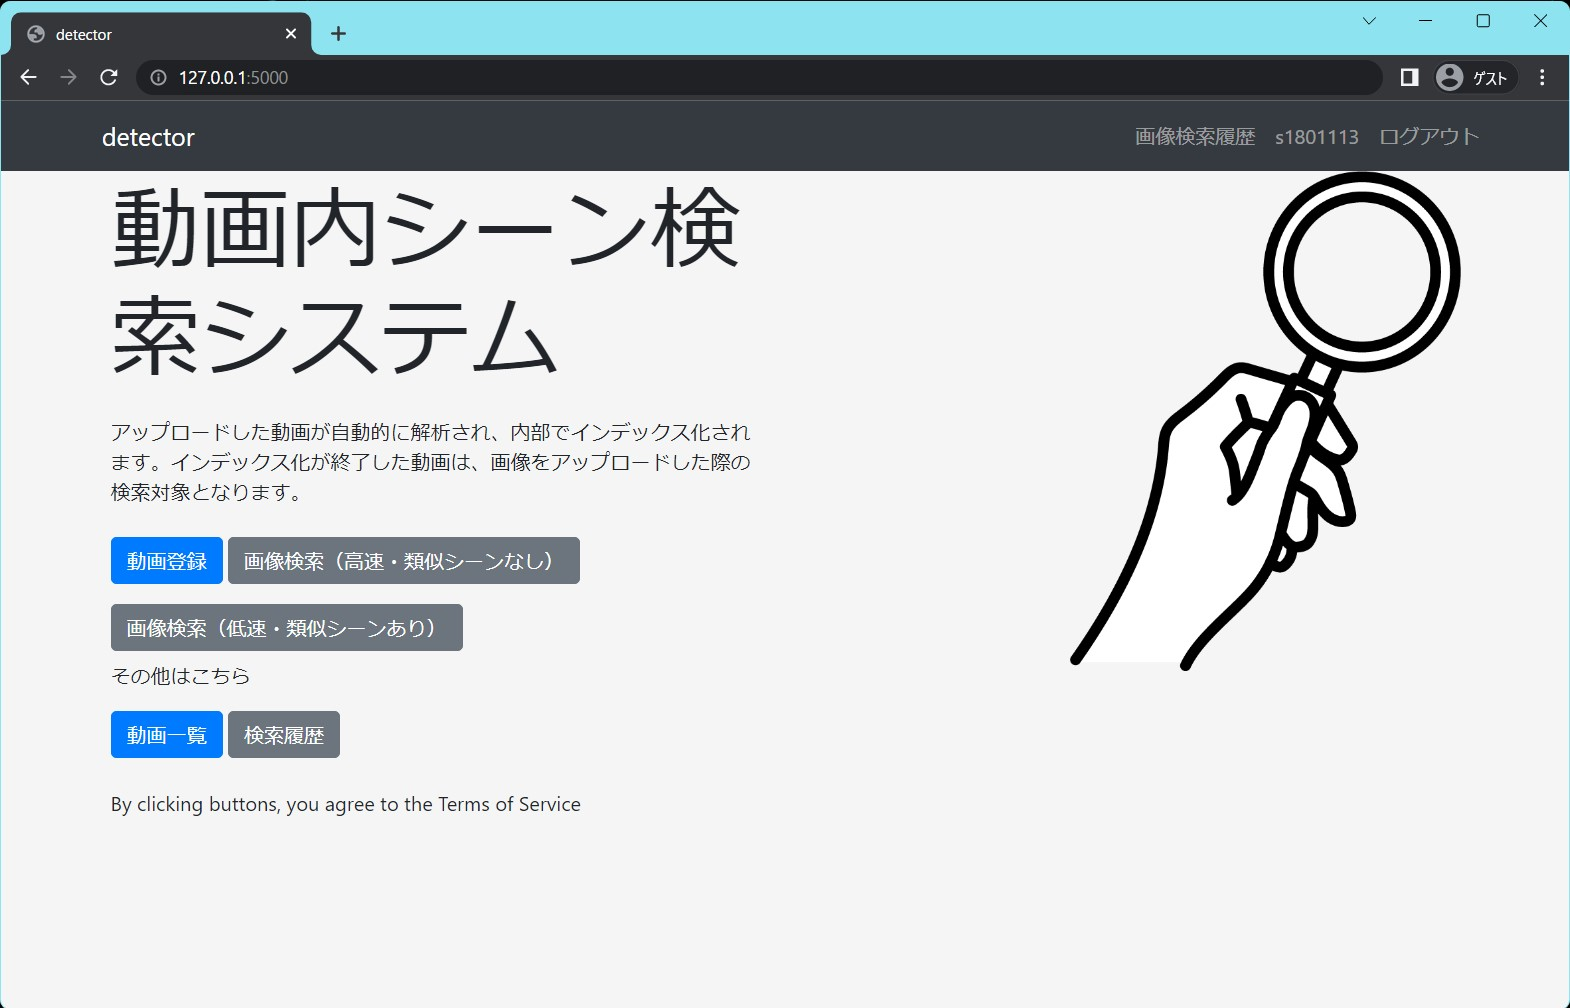
\includegraphics[width=13cm]{image/index.jpg}
  \caption{トップ画面}
  \label{fig:index}
\end{figure}

次に遷移後のアップロード画面を図\ref{fig:movie_upload}に示す.

\begin{figure}[H]
  \centering
  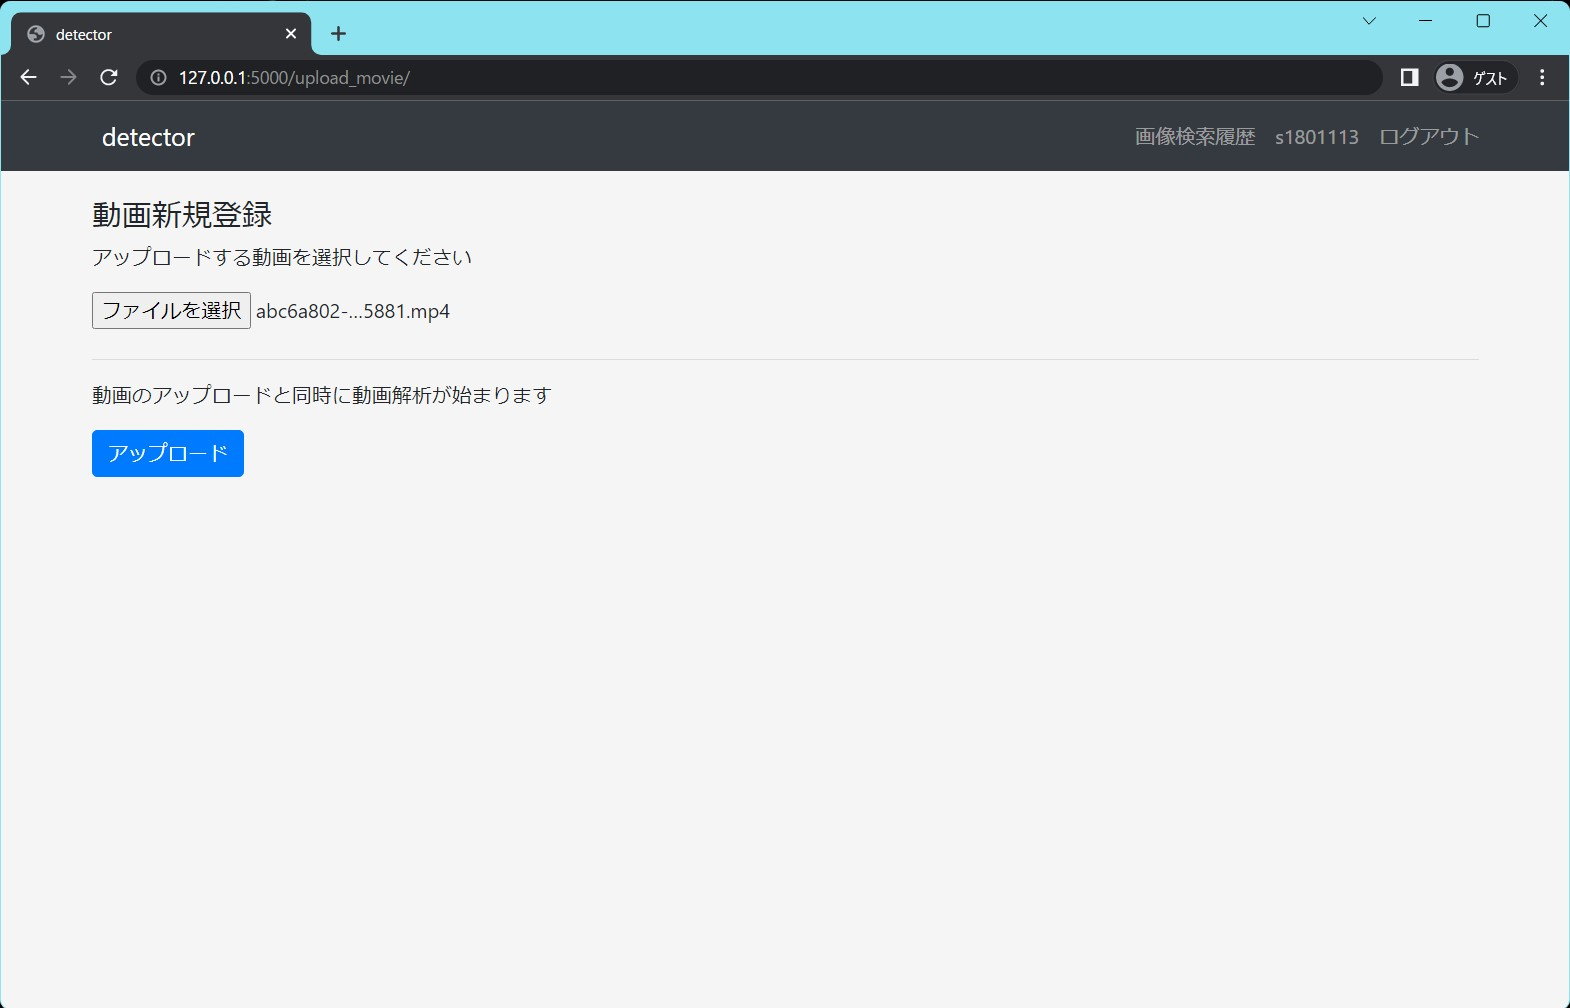
\includegraphics[width=13cm]{image/movie_upload.jpg}
  \caption{動画アップロード画面遷移後}
  \label{fig:movie_upload}
\end{figure}

その後,解析対象とする動画を選択し,アップロードを行う.
アップロードが正しく完了すると,自動的に動画リストに遷移し,解析が開始される.
複数の動画を解析対象にすることが可能だが,実際に同時には解析されず解析待ちという形で追加される.
なお,動画のアップロードが正しく完了していれば,解析待ちや解析中であってもブラウザを更新したり閉じたりしても動画には影響はない.

\section{動画データの情報表示}
動画アップロードが完了した動画は,トップ画面(図\ref{fig:index})の『動画一覧』で一覧表示される.

動画一覧,動画の解析状況および動画の解析結果を確認できる.
動画の解析が始まっていない時は,図\ref{fig:preparation}のように表示される.
\begin{figure}[H]
  \centering
  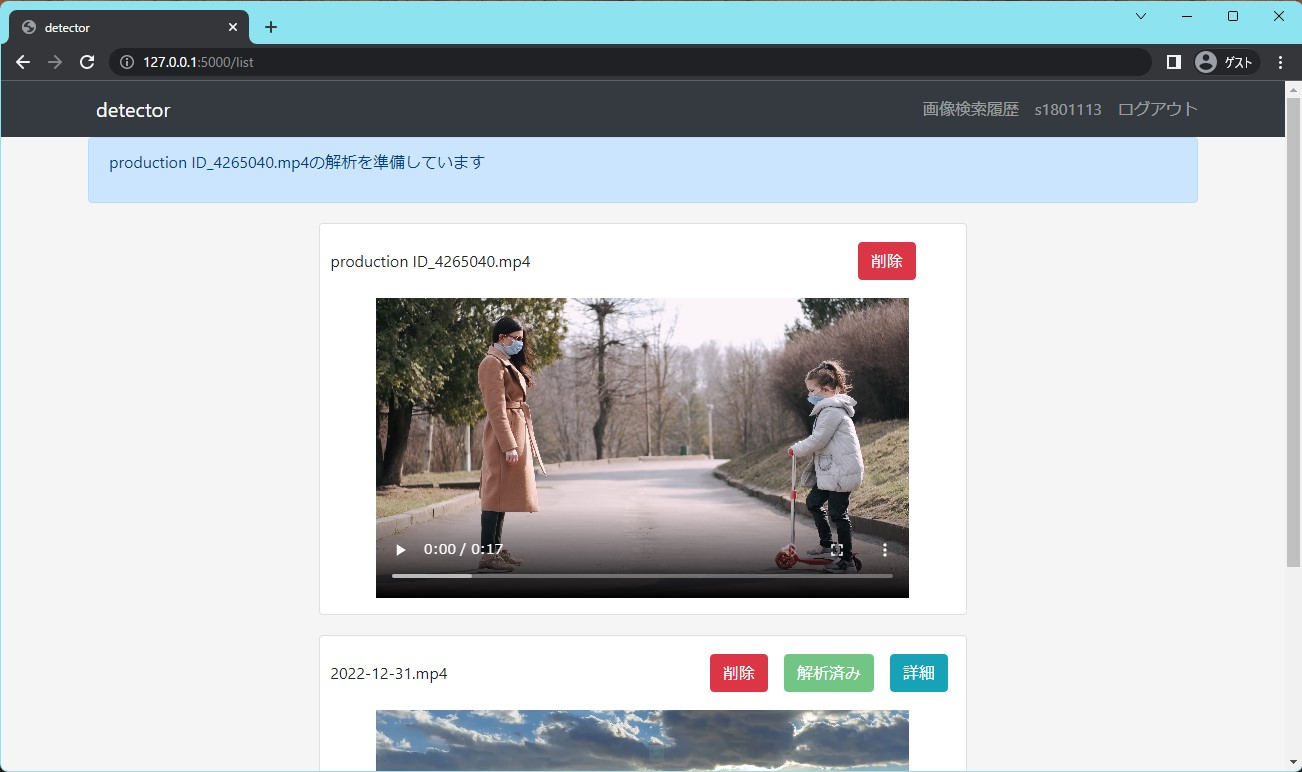
\includegraphics[width=13cm]{image/preparation.jpg}
  \caption{動画リスト(解析前)}
  \label{fig:preparation}
\end{figure}

動画は自動的に解析が行われる.画面を更新すると最新の解析状況を確認することができる(図\ref{fig:ongoing}).
\begin{figure}[H]
  \centering
  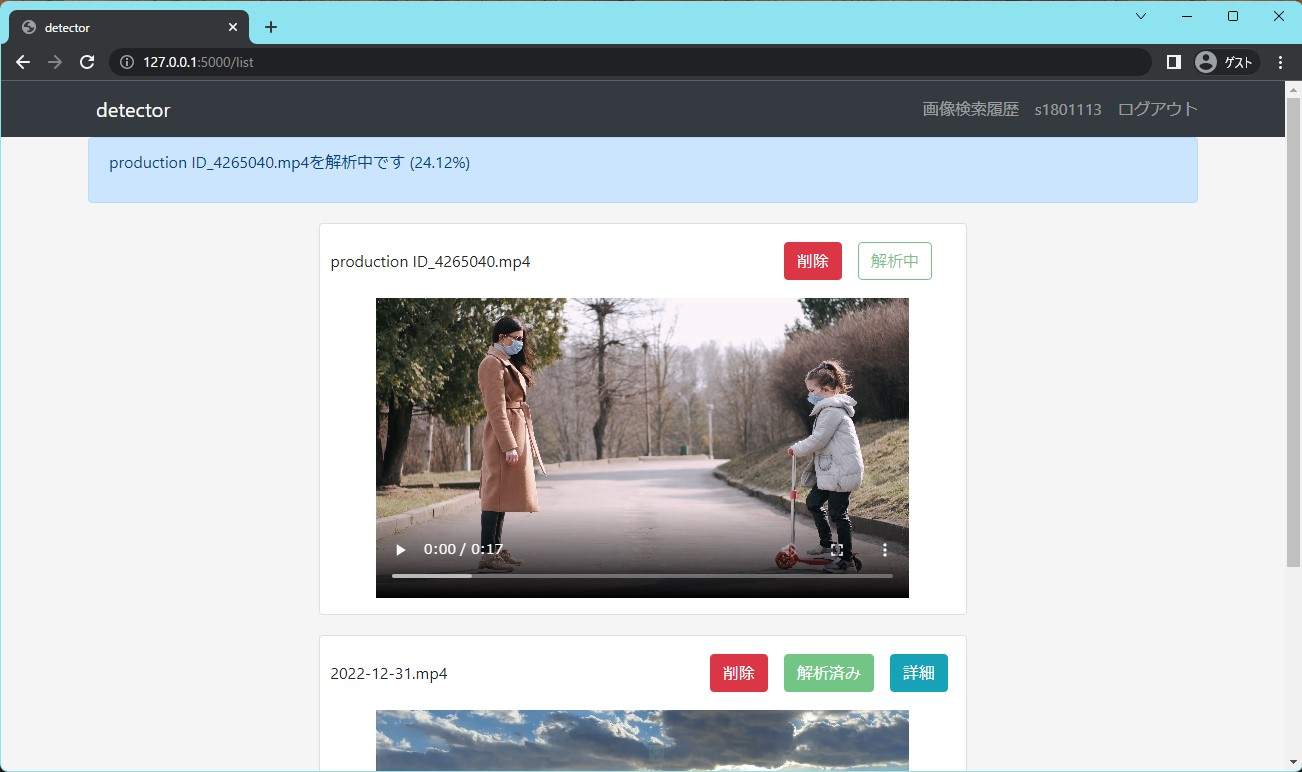
\includegraphics[width=13cm]{image/ongoing.jpg}
  \caption{動画リスト(解析中)}
  \label{fig:ongoing}
\end{figure}

解析が完了した動画は,図\ref{fig:complete}のように『解析済み』と表示される.
また,『詳細』ボタンが押せるようになり,解析状況を確認できる.
\begin{figure}[H]
  \centering
  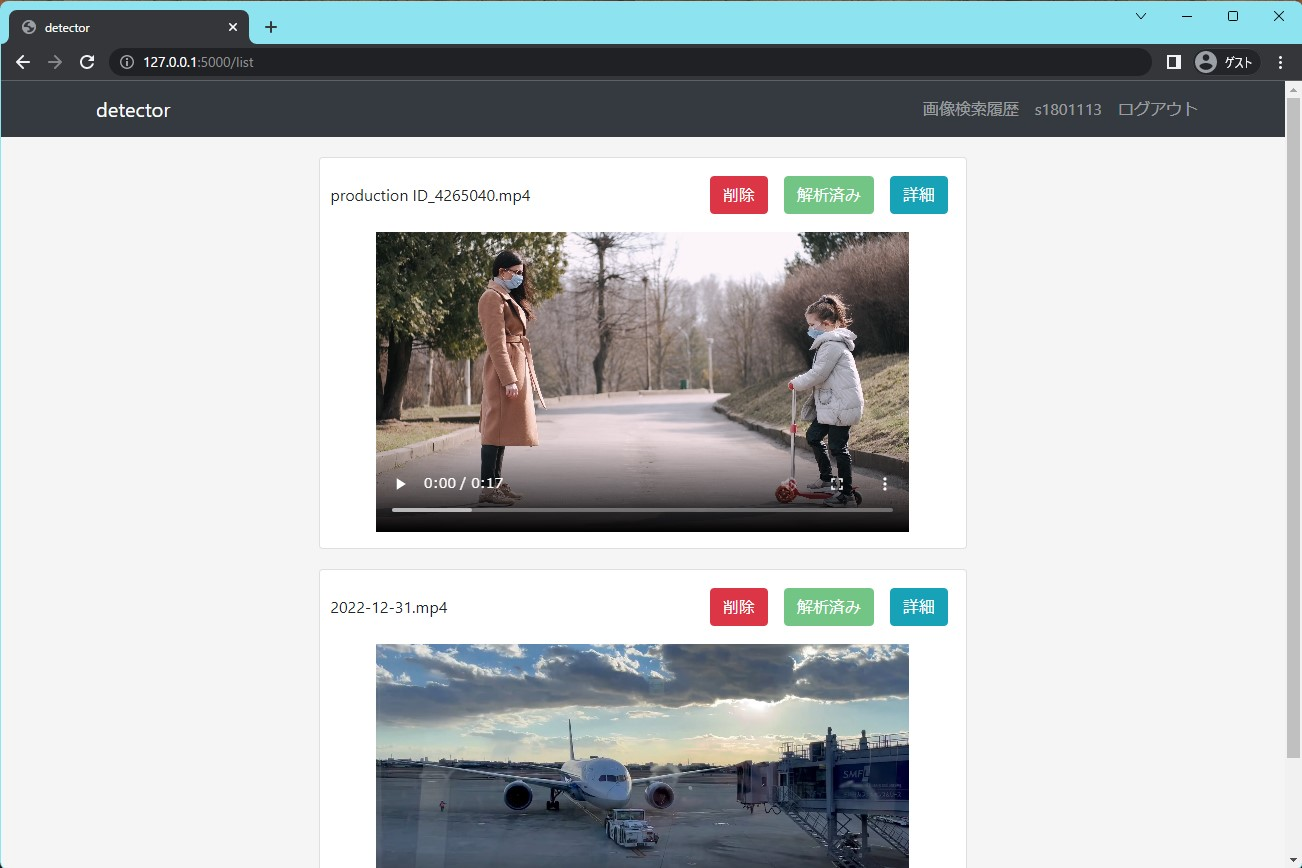
\includegraphics[width=13cm]{image/complete.jpg}
  \caption{動画リスト(解析済み)}
  \label{fig:complete}
\end{figure}

詳細ボタンを押すと,図\ref{fig:detail}のようなページに遷移する.
\begin{figure}[H]
  \centering
  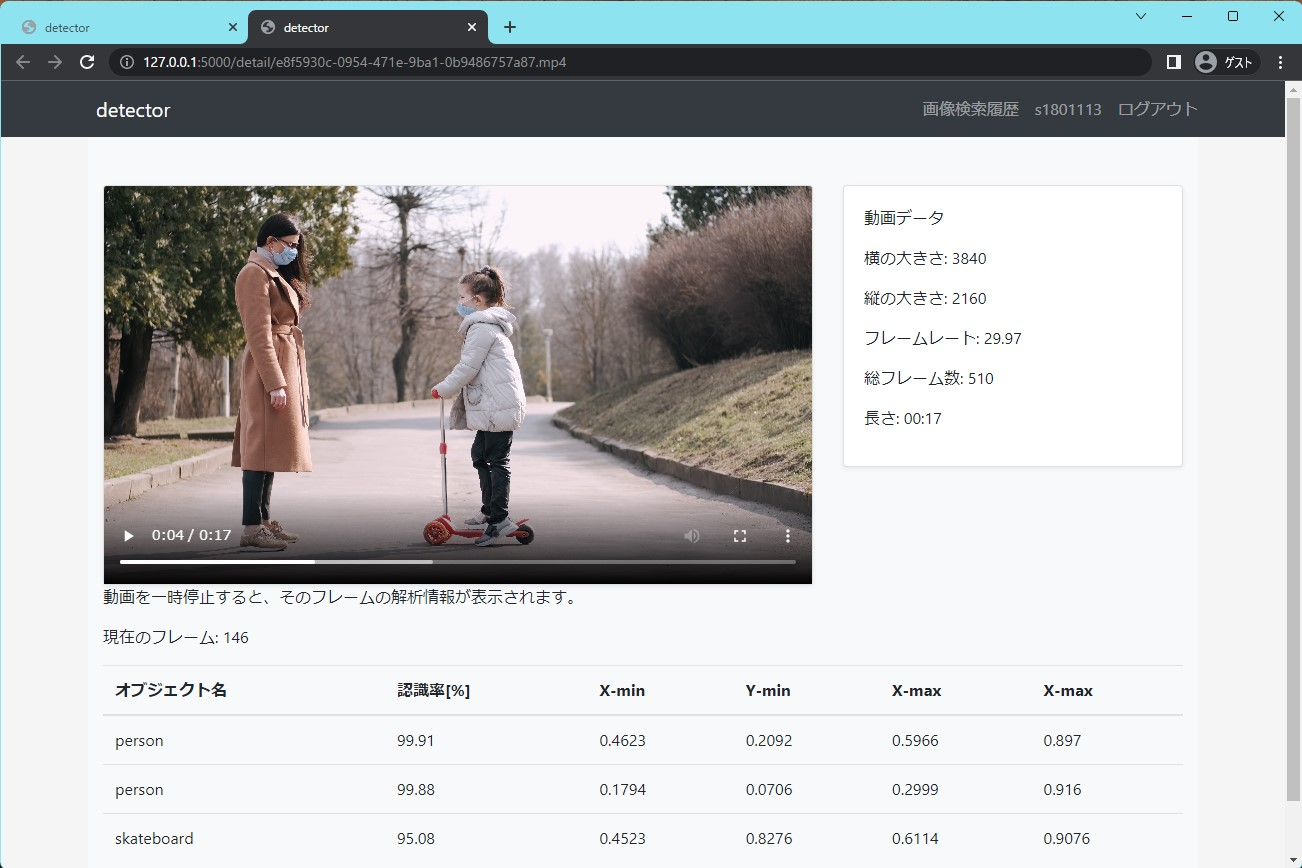
\includegraphics[width=13cm]{image/detail.jpg}
  \caption{動画データ}
  \label{fig:detail}
\end{figure}

動画のシーケンスバー(再生位置)を操作することで,目的のフレームがどのような解析結果になっているか確認できる.
また,動画のサイズや長さなど基本的なデータが画面右側に表示される.

\section{画像を用いた検索について}
動画アップロードで解析まで完了した動画は,画像を用いた検索対象となる.検索手順について説明する.

トップ画面から検索画面に遷移する図\ref{fig:index}を示す.
検索には,類似シーンの検索の有無が選択できる.

トップ画面から画像検索を選択,動画を選択した時と同様に画像を選択すると図\ref{fig:image_upload}のようになる.

\begin{figure}[H]
  \centering
  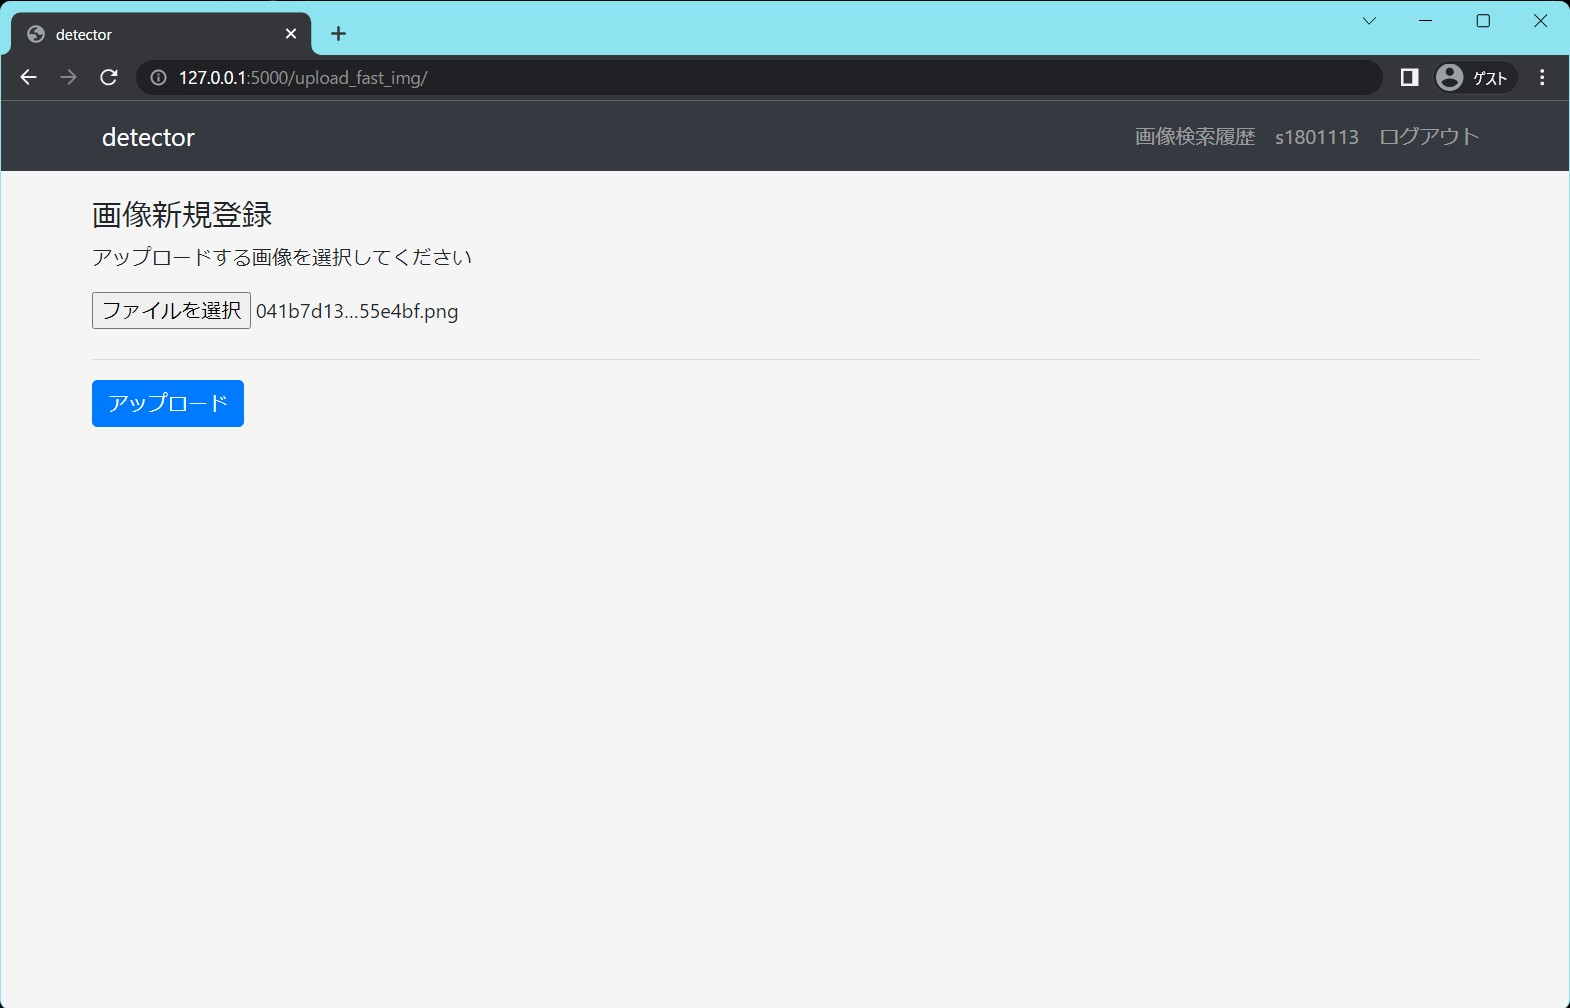
\includegraphics[width=13cm]{image/image_upload.jpg}
  \caption{画像アップロード画面遷移後}
  \label{fig:image_upload}
\end{figure}


その後,検索ボタンを選択すると,検索が開始される.
検索が終了すると,図\ref{fig:search_result}結果が表示される.

\begin{figure}[H]
  \centering
  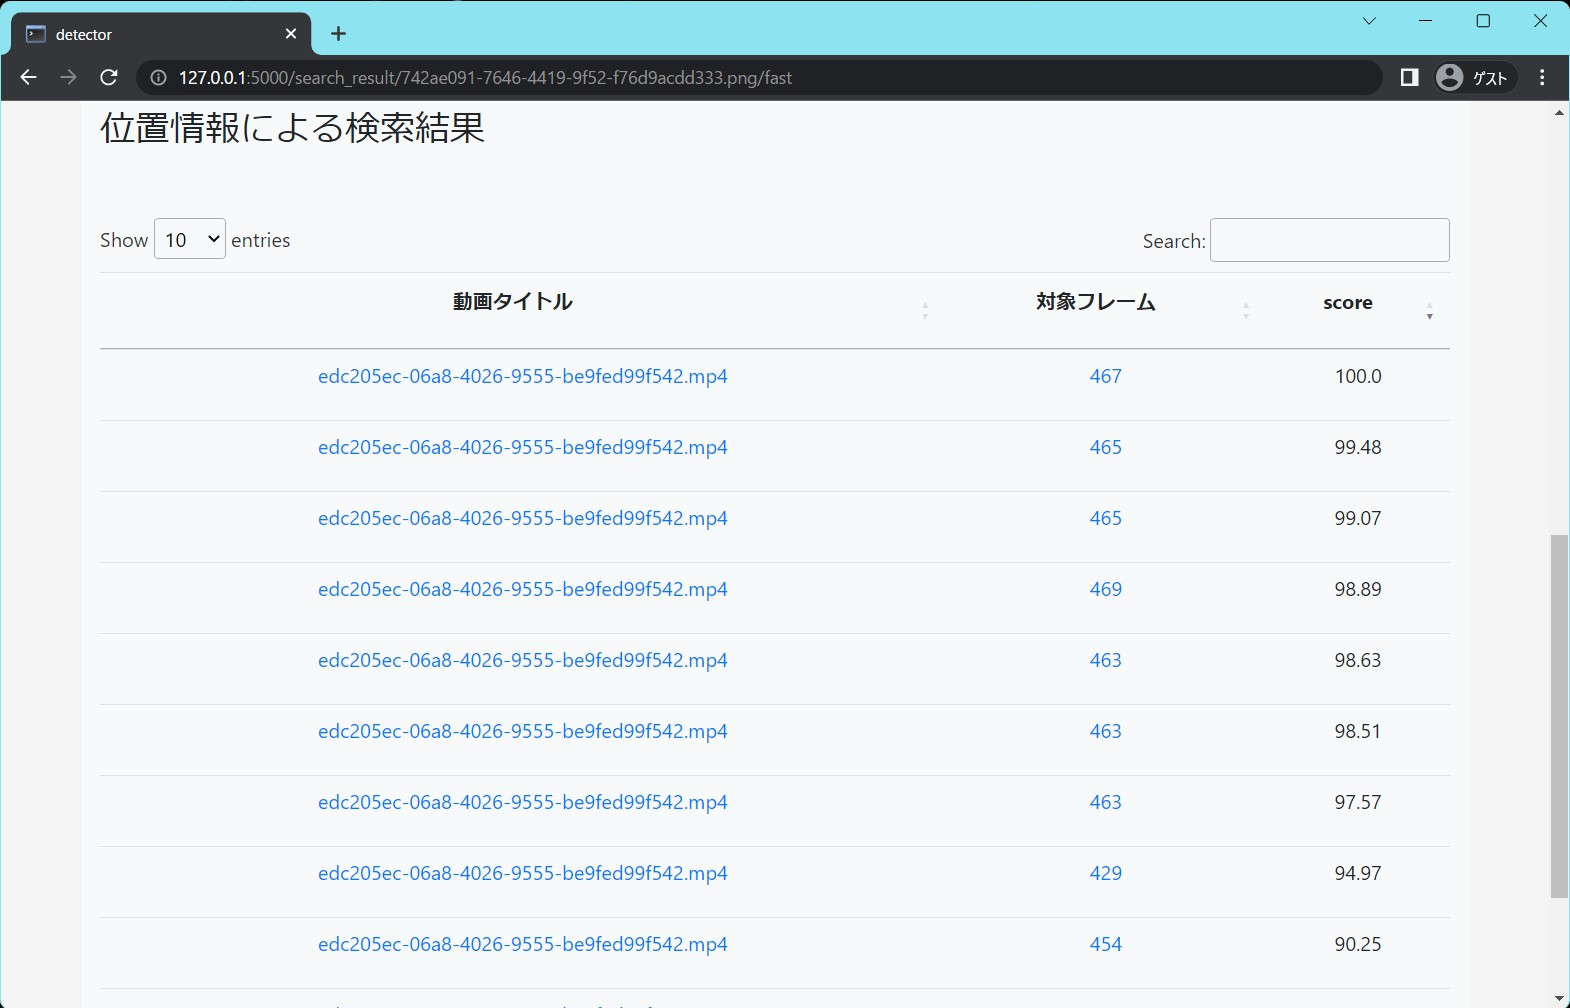
\includegraphics[width=13cm]{image/search_result.jpg}
  \caption{検索結果}
  \label{fig:search_result}
\end{figure}


この結果画面から,どの画像のどのシーン(フレーム)がどの程度類似しているかを確認することが可能になっている.
詳細な情報については,動画フレーム数のリンクから閲覧できる.ここでは,どのように認識されているかを確認でき,実際の動画を視聴することが可能となっている.

また,一度検索した画像は検索履歴として残っているため後から同じ画像を検索することが可能である.ヘッダー「画像検索履歴」を選択することで履歴が表示される.

\end{document}
